\documentclass[12pt, reqno]{amsart}
\usepackage[margin = 0.5 in]{geometry}
\usepackage{multicol}
\usepackage{float}
\usepackage{fancyhdr}
\usepackage{graphicx}
\usepackage{hyperref}
\usepackage{fancyvrb}
\usepackage{physics}
\raggedbottom

\frenchspacing

\setlength{\abovecaptionskip}{5pt plus 3pt minus 3pt}

\hypersetup{colorlinks=true,allcolors=blue}
\pagestyle{fancy} \fancyhead{} \fancyfoot[C]{\normalsize\thepage}
\renewcommand{\headrulewidth}{0pt}
\begin{document}
\title{ME 5311 \quad Project Extra Credit \quad Jacob Ivanov}

\maketitle
\section{Tridiagonal Convergence}
\begin{figure}[H]
    \centering
    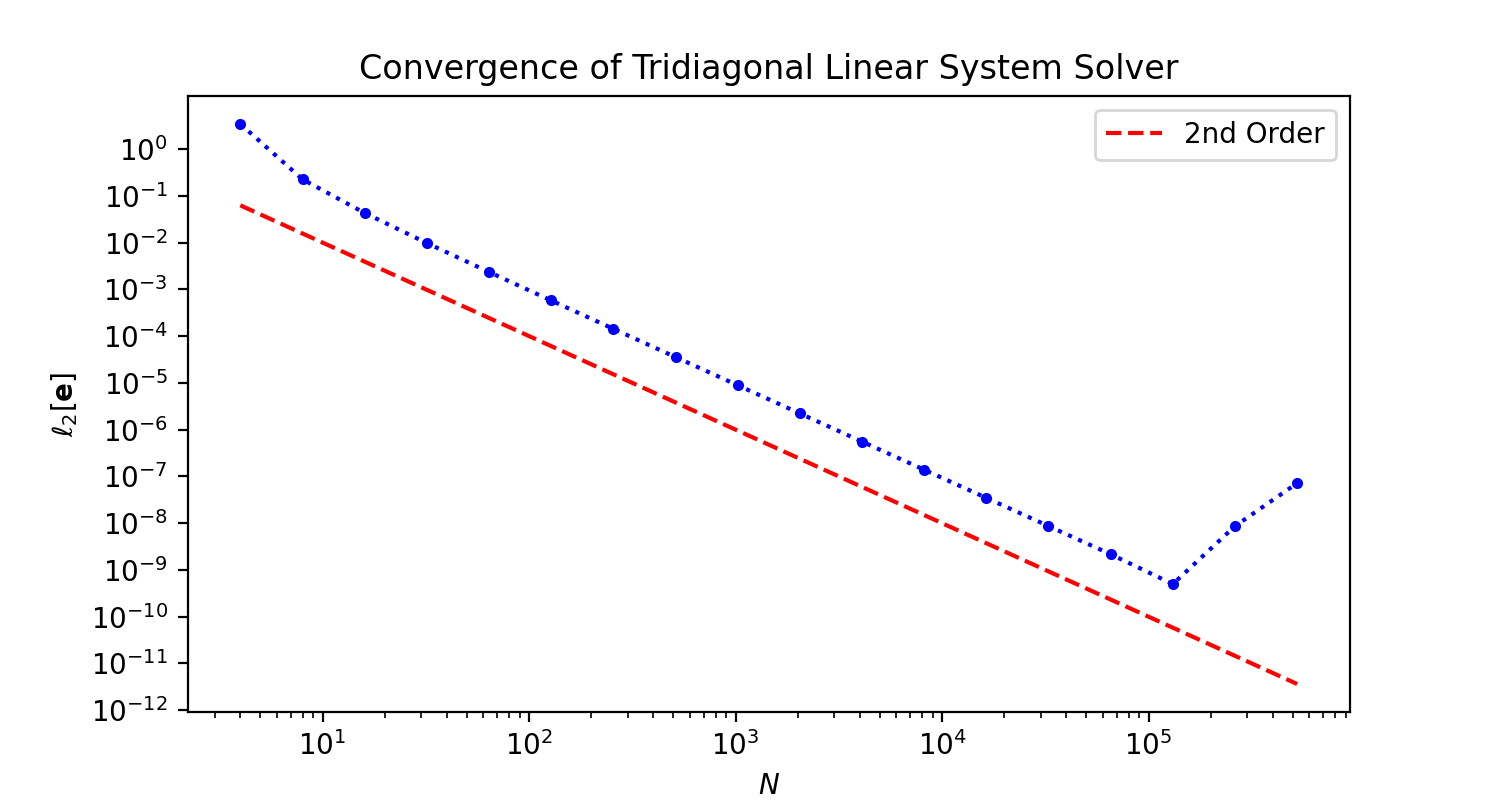
\includegraphics[width=1\linewidth]{tridiagonal_convergence.png}
\end{figure}

\section{Fourier Method Convergence}
\begin{figure}[H]
    \centering
    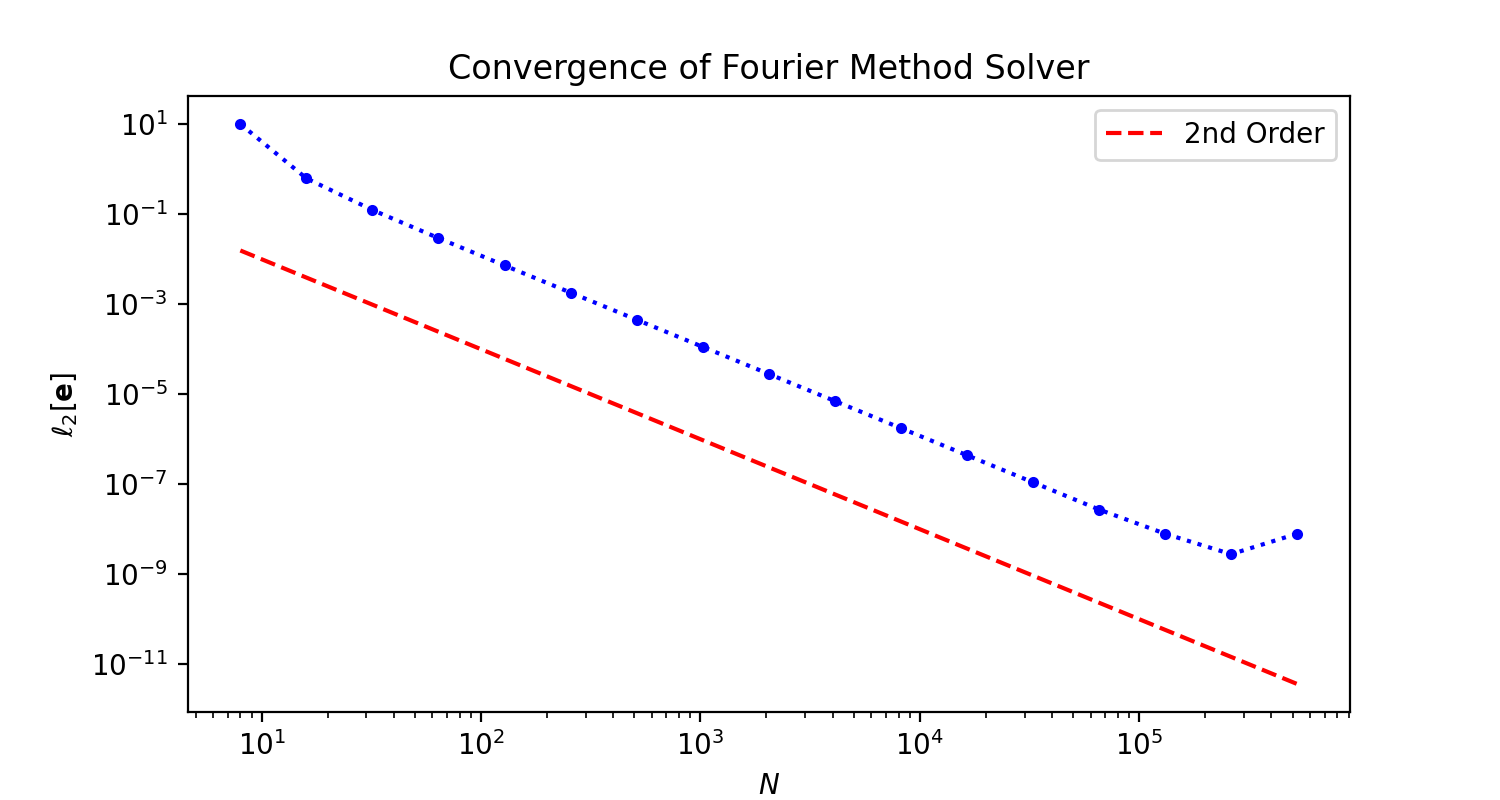
\includegraphics[width=1\linewidth]{fourier_convergence.png}
\end{figure}

\end{document}